\appendix{Computer Aided Analytical Solutions}\label{app:math}


% This LaTeX was auto-generated from MATLAB code.
% To make changes, update the MATLAB code and republish this document.

MATLAB was used to solve analytical models for the air gap sensor during the sensor's design.
The resulting performance graphs are shown in \ref{fig:appc_airgap_graph}.
The graphs shows performance near the empircally measured value of 10 Newton per Hertz.
The model has many parameters, so the uncertainty is collected in the parasitic capaciance and inductance.
The overall device stiffness is also adjusted for this model, to a value of 6 GN/m.
This limits the strain in the model to the feasible region of the air gap.
The equation for Hertz per Newton is found by the script, and is given in \ref{eq:air_gap_sense_c}
The script and output are given in \ref{lst:airgap1} and \ref{lst:airgap2}, respectively.

\begin{figure}[ht]
\centering
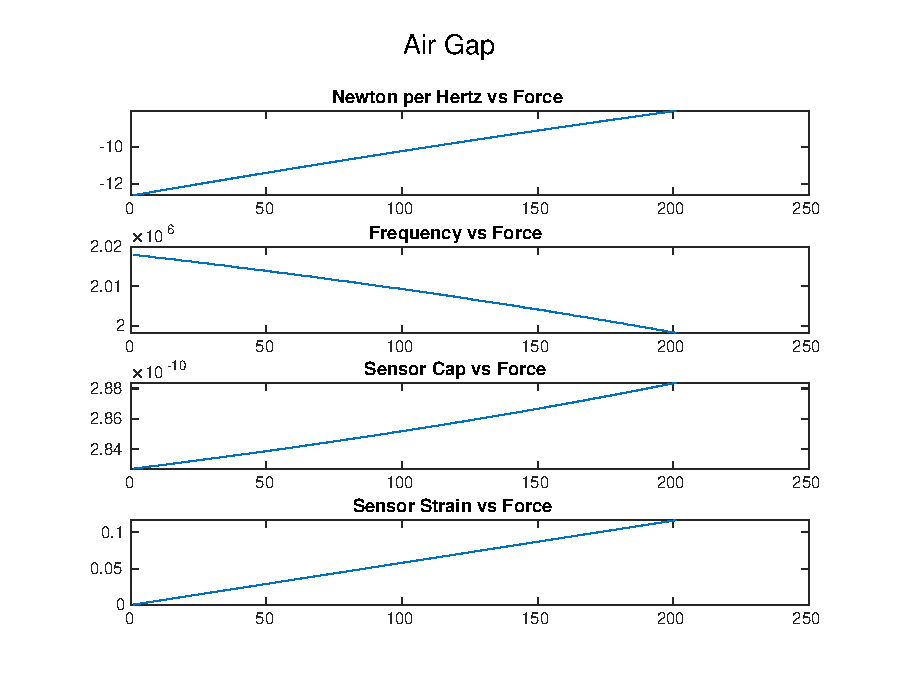
\includegraphics[width=0.6\textwidth]{appc_air_gap_plot.eps}
\caption{
Result of computation of device frequency and sensitivity over the required input range.
}
\label{fig:appc_airgap_graph}
\end{figure}

\begin{equation}\label{eq:air_gap_sense_c}
 \frac{df}{dF} = 
-\frac{0.0796\,A\,L\,e_{1}\,{e_{2}}^2}{\mathrm{ks}\,{\left(2.5000e-05\,e_{1}+e_{2}\,\left(\mathrm{d1n}-\frac{F}{\mathrm{ks}}\right)\right)}^2\,{\left(L\,\left(\mathrm{cb}+\frac{A\,e_{2}}{\mathrm{d2n}}+\frac{A\,e_{1}\,e_{2}}{2.5000e-05\,e_{1}+e_{2}\,\left(\mathrm{d1n}-\frac{F}{\mathrm{ks}}\right)}\right)\right)}^{1.5000}}
\end{equation}    

\pagebreak



%% Closed Area
A model was also used to explore the closed area sensor configuration. 
The resulting performance graphs are shown in \ref{fig:appc_closed_graph}.
The sensitivity is much greater for this model, requiring less Newtons to 
alter the resonant frequency in Hertz when compared to the air gap model.
For these calculations, the sensitivity can approach infinity as the region size
approaches zero. In reality, the device will continue to get stiffer as it compresses 
considerably, limiting the compression. The equation for the sensitivity to input force
is shown in \ref{eq:appc_d1}. The true sensor does not have completly linear characteristics,
but the sensitivity increases with greater force. Also, the sensitivity is approximately linear
with input force, so the response is roughly proportional to the square of the input force
for this configuration.
This model does not entirely capture the performance of the sensor during the rock cutting experiment,
but agrees with the trend that a more compressed sensor is more sensitive, 
and it shows sensitivity of similar magnitude.
The script and output are given in \ref{lst:closed1} and \ref{lst:closed2}, respectively.


\begin{figure}[ht]
\centering
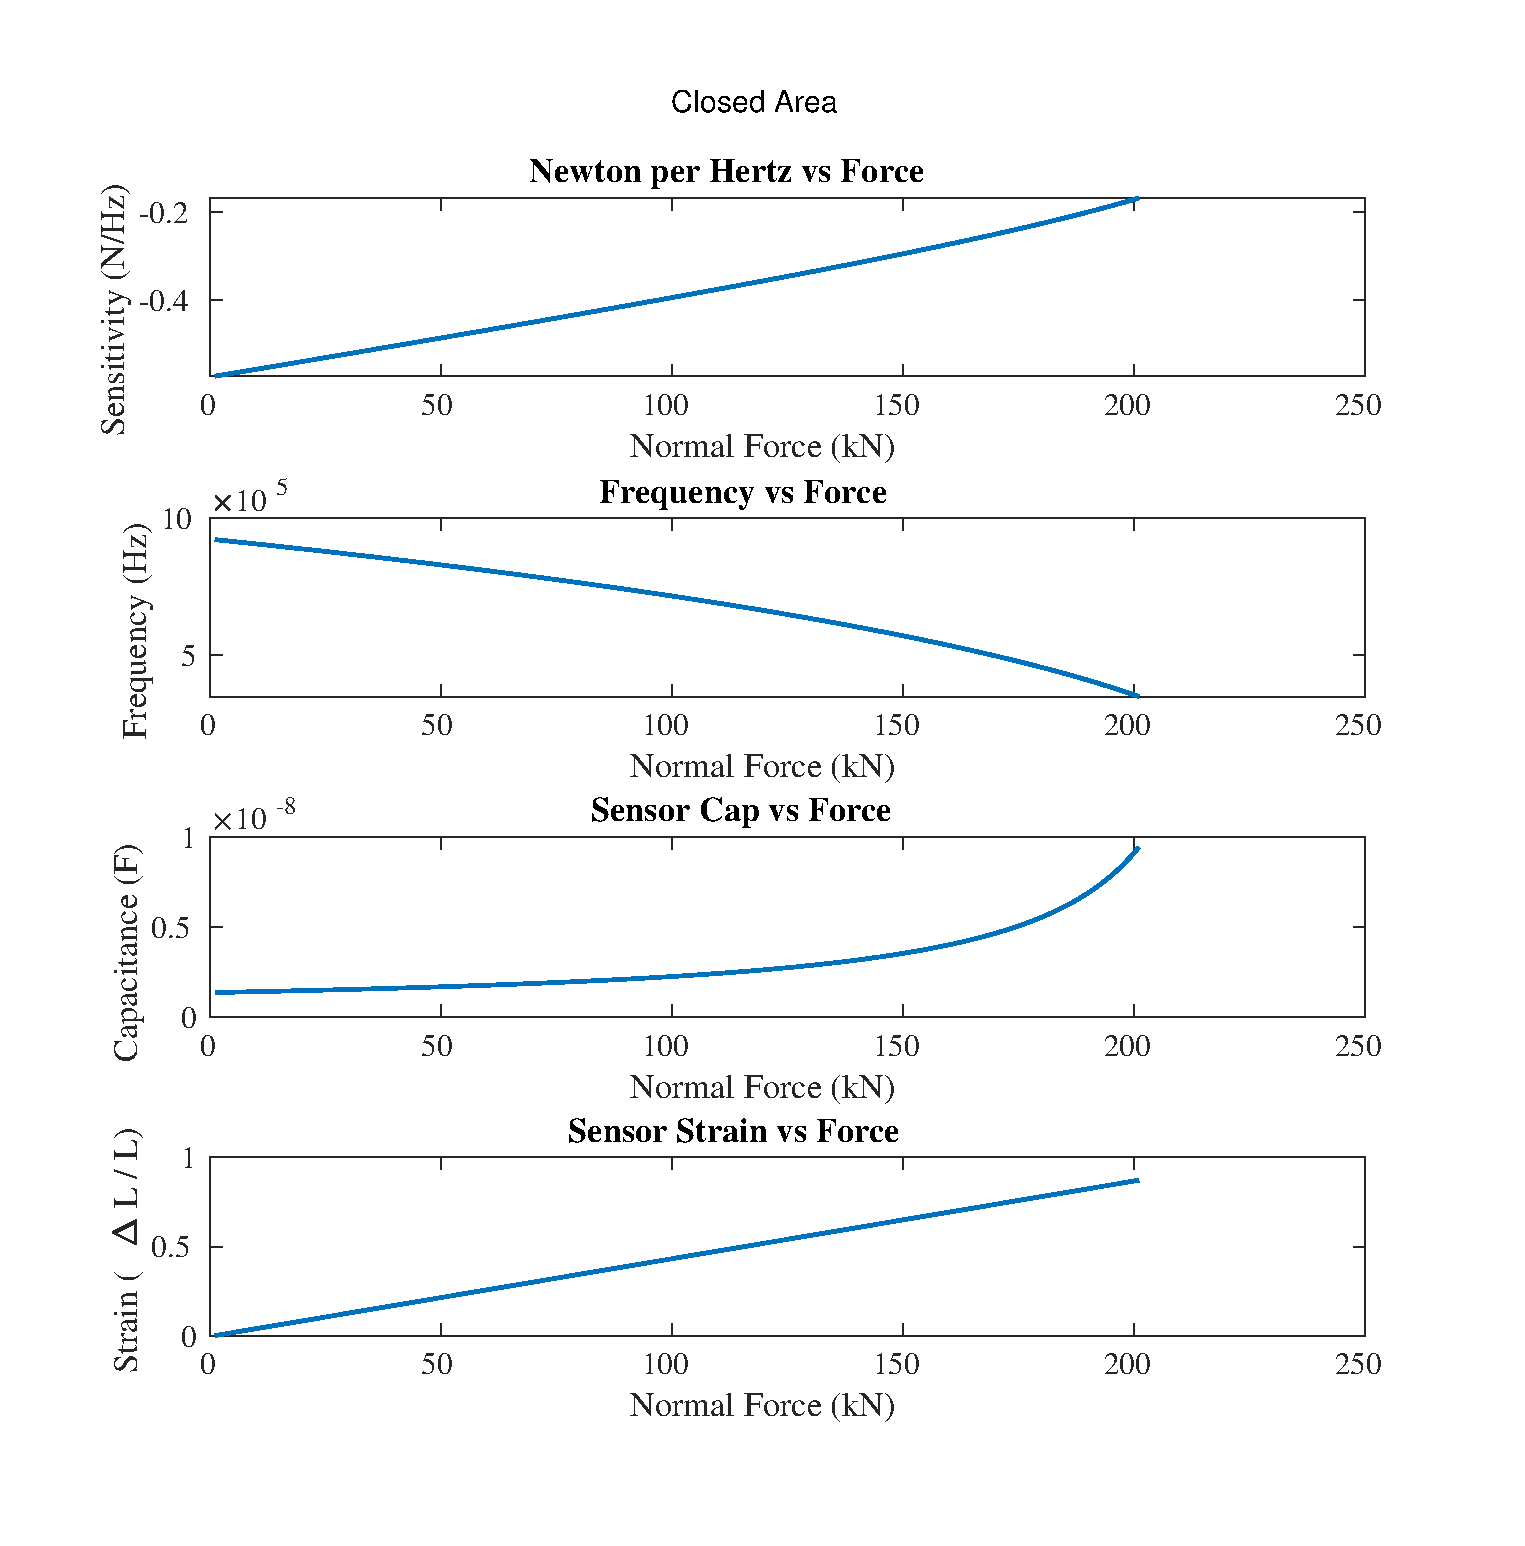
\includegraphics[width=0.6\textwidth]{appc_closed_gap_plot.eps}
\caption{
Result of computation of device frequency and sensitivity over the required input range.
}
\label{fig:appc_closed_graph}
\end{figure}

\begin{equation} \label{eq:appc_d1}
\frac{df_{r1}}{dF} = -\frac{0.0796\,L\,\left(\frac{A\,e}{k_{1}\,{\left(\mathrm{d1n}-\frac{F}{k_{1}}\right)}^2}+\frac{A\,e}{k_{2}\,{\left(\mathrm{d2n}-\frac{F}{k_{2}}\right)}^2}\right)}{{\left(L\,\left(\mathrm{cb}+\frac{A\,e}{\mathrm{d1n}-\frac{F}{k_{1}}}+\frac{A\,e}{\mathrm{d2n}-\frac{F}{k_{2}}}\right)\right)}^{1.5000}}
\end{equation}

\pagebreak

%% listings

\lstinputlisting[language=Matlab,label={lst:airgap1},caption={Script for modelling air gap}]{supporting-files/matlabs/airgap_script.m}

\pagebreak

\lstinputlisting[language=Matlab,label={lst:airgap2},caption={Output from air gap script}]{supporting-files/matlabs/airgap_output.txt}

\pagebreak

\lstinputlisting[language=Matlab,label={lst:closed1},caption={Script for modelling closed area}]{supporting-files/matlabs/closed_script.m}

\pagebreak

\lstinputlisting[language=Matlab,label={lst:closed2},caption={Output from closed area script}]{supporting-files/matlabs/closed_output.txt}

